% !TeX root = induction-he.tex

\chapter{%
פתרונות%
}\label{a.solutions}

\setlength{\jot}{6pt}

\begin{enumerate}
\item 
\[
\sum_{i=1}^4 i = \sum_{i=1}^3 i + 4 \ih{} \frac{3(3+1)}{2} + 4 = \frac{20}{2} = \frac{4(4+1)}{2}\,.
\]

\item
טענת בסיס:
$1^2 = 1 = \frac{1}{6}\cdot 2\cdot 3$.
צעד אינדוקטיבי:
\begin{eqnarray*}
\sum_{i=1}^{n+1} i^2 &=& \sum_{i=1}^n i^2 + (n+1)^2\\
&\ih{}& \frac{n}{6}(n+1)(2n+1) + (n+1)^2\\
&=& \frac{(n+1)}{6} (n(2n+1) + 6(n+1))\\
&=& \frac{(n+1)}{6}(2n^2+7n+6)\\
&=& \frac{(n+1)}{6}(n+2)(2n+3)\\
&=& \frac{(n+1)}{6}((n+1)+1)(2(n+1)+1)\,.
\end{eqnarray*}

\item 
טענת בסיס:
$2\cdot 1! = 2 \geq 2^1 = 2$.
צעד אינדוקטיבי:
\[
2(n+1)!=2n!(n+1)\ihge{}2^n(n+1) \geq 2^n(2) = 2^{n+1}\,,
\]
בגלל ש-%
$n\geq 1$
ולכן
$n+1 \geq 2$.

\item
טענת בסיס:
$1\cdot 2 \cdot 3 = 6$
מתחלק ב-%
$3$.
צעד אינדוקטיבי: לפי הנחת האינדוקציה
$n(n+1)(n+2)$
מתחלק ב-%
$3$.
אם
$(n+1)$
או
$(n+2)$
מתחלק ב-%
$3$.
גם 
\[
(n+1)((n+1)+1)((n+1)+2)
\]
מתחלק ב-%
$3$.
אחרת,
$n$
מתחלק ב-%
$3$
ו-%
$n=3k$.
מכאן ש:
\[
(n+1)+2 = n+3=3k+3=3(k+1)
\]
מתחלק ב-%
$3$.

\item
טענת בסיס:
$1^3-1=0$
מתחלק ב-%
$6$.
צעד אינדוקטיבי:
\[
n^3-n=n(n^2-1)=n(n+1)(n-1)=(n-1)n(n+1)\,.
\]
לפי תרגיל~%
\ref{e.div3},
אחד מתוך
$(n-1),n,(n+1)$
מתחלק ב-%
$3$.
אם
$n-1$
מתחלק ב-%
$3$
אז לפי משפט~%
\ref{t.div2} $n(n+1)$
מתחלק ב-%
$2$,
ולכן המכפלה מתחלקת ב-%
$6$.
באופן דומה, אם
$n+1$
מתחלק ב-%
$3$
אז
$(n-1)n$
מתחלק ב-%
$2$,
ולכן המכפלה מתחלקת ב-%
$6$.
לבסוף, אם
$n$
מתחלק ב-%
$3$,
או ש-%
$n$
הוא גם זוגי ולכן מתחלק ב-%
$6$,
או שהוא אי-זוגי וגם
$n-1$
ו-%
$n+1$
זוגיים ומתחלקים ב-%
$2$,
כך שהמכפלה מתחלקת ב-%
$6$.

\item
טענת בסיס: עבור
$n=1$,
ברור שלא ניתן לשים 
$1+1=2$
יונים בתא אחד כך שיש לכל היותר יונה אחת בתא. צעד אינדוקטיבי: נתונים 
$n+1$
יונים ו-%
$n$
תאים. שים יונה אחת בתא שרירותי. אסור לשים יונה נוספת באותו תא, לכן נשארו לנו 
$n$
יונים שיש לשים ב-%
$n-1$
תאים. לפי הנחת האינדוקציה הדבר בלתי אפשרי.

\item
נבדוק את האי-שוויון למספר ערכים קטנים:
\begin{eqnarray*}
2^1=2&\geq& 1^2 = 1\,,\\
2^2=4&\geq& 2^2 = 4\,,\\
2^3=8&\not\geq& 3^2 = 9\,,\\
2^4=16&\geq& 4^2 = 16\,,\\
2^5=32&\geq& 5^2 = 25\,.
\end{eqnarray*}
נראה שהנוסחה נכונה עבור כל מספר פרט ל-%
$n=3$.
אז ניקח בטענת הבסיס את הערך
$n=4$.

הצעד האינדוקטיבי הוא:
\[
2^{n+1}=2^n\cdot 2 \ihge{} n^2\cdot 2 = n^2 + n^2 \stackrel{?}{\geq} n^2 + 2n + 1 = (n+1)^2\,.
\]
הצעד האינדוקטיבי נכון עבור 
$n$
כאשר
$n^2\geq 2n+1$,
כלומר עבור
$n>2$.

מכאן אנו מבינים מדוע אי-אפשר להוכיח את הנוסחה באינדוקציה עבור טענת בסיס לערך
$n=2$.
הצעד האינדוקטיבי מ-%
$n=2$
ל-%
$n+1=3$
לא עובד.

\item 
טענת בסיס:
$2=1(1+1)$.
הצעד האינדוקטיבי הוא:
\[
\sum_{i=1}^{n+1} 2i = \sum_{i=1}^n 2i + 2(n+1) \ih{} n(n+1) + 2(n+1)= (n+1)(n+2)\,.
\]

\item
הוכחת טענת הבסיס זהה להוכחה עבור משפט~%
\ref{th.three}.
הצעד האינדוקטיבי הוא:
\begin{eqnarray*}
\overbrace{kkk}^{3^{n+1}} &=& \overbrace{kkk}^{3^n}\cdot\overbrace{kkk}^{3^n}\cdot \overbrace{kkk}^{3^n}\\
&\ih{}&(3^nm)10^{2\cdot 3n} + (3^nm)10^{3n} + (3^nm)\\
&=&(3^nm)(10^{2\cdot 3n} + 10^{3n} + 1)\,.
\end{eqnarray*}
חילוק של כל חזקה של 
$10$
על ידי
$3$
משאיר שארית של
$1$,
לכן
$(10^{2\cdot 3n} + 10^{3n} + 1)$
מתחלק ב-%
$3$
ו-
$(3^nm)(10^{2\cdot 3n} + 10^{3n} + 1)$
מתחלק ב-%
$3^{n+1}$.

\item
טענת בסיס:
$a_1=5=3+2^1$, $a_2=7=3+2^2$.
הצעד האינדוקטיבי הוא:
\begin{eqnarray*}
a_{n+1}&=&3a_{n+1-1}-2a_{n+1-2}\\
&\ih{}&3(3+2^n)-2a_{n+1-2}\\
&\ih{}&3(3+2^n)-2(3+2^{n-1})\\
&=&9 + 3\cdot 2^n-6-2^n\\
&=&3+2\cdot 2^n\\
&=&3+2^{n+1}\,.
\end{eqnarray*}
\item 
יהי
$S=\{x = an_1+bn_2: x>0\}$.
בגלל ש-%
$S$
היא קבוצה לא ריקה, לפי עיקרון הסדר הטוב קיים איבר קטן ביותר
 $d\in S$,
כאש
$d=a'n_1+b'n_2>0$.
לפי אלגוריתם החלוקה:
\begin{eqnarray*}
n_1&=&qd+r,\;\;\; \mathrm{for}\;0\leq r < d\\
r &=& n_1-qd\\
&=& (1-qa')n_1+(-b'q)n_2\,,
\end{eqnarray*}
כך ש-%
$r\in S$.
אבל לא ייתכן
$0<r<d$
כי
$d$
הוא האיבר הקטן ביותר ב-%
$S$,
ולכן
$r=0$
ו-%
$d\mid n_1$.
הוכחה דומה מראה ש-%
$d\mid n_2$,
ולכן
$d$
הוא מחלק משותף של
$n_1,n_2$.
אם 
$c$
הוא מחלק משותף כלשהו של
$n_1, n_2$,
$c\mid (a'n_1+b'n_2)=d$,
ומכאן ש-%
$d=\gcd(n_1,n_2)$.

\item
יהי
$p \mid n_1n_2$ 
והנח ש-%
$p$
\textbf{לא מחלק}
את
$n_1$.
מכאן ש-%
$p$
ו-%
$n_1$
הם ראשוניים אחד לשני. לפי הזהות של 
\L{Bezout}
קיימים
$a,b$
כך ש-%
$an_1+bp=1$.
נכפיל ב-%
$n_2$
ונקבל:
\[
an_1n_2 + bpn_2 = n_2\,.
\]
לפי ההנחה
$p \mid n_1n_2$
אז
$p \mid an_1n_2$
וברור ש-%
$p \mid bpn_2$
ולכן
$p\mid n_2$.

\item
טענת בסיס:
$a_1=2=1(1+1)$.
הצעד האינדוקטיבי הוא:
\[
\sum_{i=1}^{n+1}a_i=\sum_{i=1}^n a_i+a_{n+1}\ih{}n(n+1)+a_{n+1}=n(n+1)+2(n+1)=(n+1)(n+2).
\]
נשמתמש במשפט~%
\ref{t.recursive}
כדי להציב
$2(n+1)$
במקום
$a_{n+1}$.

\item 
טענת בסיס:
$f_5=5$ 
מתחלק ב-%
$5$.
הצעד האינדוקטיבי הוא:
\begin{eqnarray*}
f_{5(n+1)} &=& f_{5n+5}\\
&=& f_{5n+4}+f_{5n+3}\\
&=& 2f_{5n+3}+f_{5n+2}\\
&=& 3f_{5n+2}+2f_{5n+1}\\
&=& 5f_{5n+1}+3f_{5n}\,.
\end{eqnarray*}
הגורם הראשון 
$5f_{5n+1}$
מתחלק ב-%
$5$
ולפי הנחת האינדוקציה
גם
$3f_{5n}$
מתחלק ב-%
$5$.

\item 
טענות בסיס:
$f_1=1<(\frac{7}{4})^1$
ו-%
$f_2=1<(\frac{7}{4})^2=\frac{49}{16}$.
הצעד האינדוקטיבי הוא:
\begin{eqnarray*}
f_{n+1}&=&f_n+f_{n-1}\\
&\ihlt{}&\left(\frac{7}{4}\right)^n + f_{n-1}\\
&\ihlt{}&\left(\frac{7}{4}\right)^n + \left(\frac{7}{4}\right)^{n-1}\\
&=&\left(\frac{7}{4}\right)^{n-1}\cdot\left(\frac{7}{4}+1\right)\\
&<&\left(\frac{7}{4}\right)^{n-1}\cdot\left(\frac{7}{4}\right)^2\\
&=&\left(\frac{7}{4}\right)^{n+1},
\end{eqnarray*}
בגלל ש-%
\[
\left(\frac{7}{4}+1\right) = \frac{11}{4} = \frac{44}{16}<\frac{49}{16}=\left(\frac{7}{4}\right)^2.
\]

\item
טענת בסיס
)$n=2$(: $F_2=2^{2^2}+1=17$.

הנחת האינדוקציה:
$F_n=10k_n+7$.

הצעד האינדוקטיבי:
\begin{eqnarray*}
F_{n+1}&=&2^{2^{n+1}}+1=\left(2^{2^{n}}\right)^2+1\\
&=&\left(\left(2^{2^{n}}+1\right)-1\right)^2+1\\
&\ih&(10k_n+7-1)^2+1=(10k_n+6)^2+1\\
&=&100k_n^2+120k_n+36+1\\
&=&10(10k_n^2+12k_n+3)+6+1\\
&=&10k_{n+1}+7\,.
\end{eqnarray*}

\item
טענת בסיס:
\[
5=F_1=\prod_{k=0}^{0} F_k + 2=F_0+2=3+2\,.
\]
הצעד האינדוקטיבי:
\begin{eqnarray*}
\prod_{k=0}^{n}F_k&=&(\prod_{k=0}^{n-1}F_k) F_n \\
&\ih& (F_n-2)F_n\\
&=& (2^{2^n}+1-2)(2^{2^n}+1)\\
&=& 2^{2^{n+1}}-1\\
&=& (2^{2^{n+1}}+1)-2\\
&=&F_{n+1}-2\\
F_{n+1}&=&\prod_{k=0}^{n}F_k + 2\,.
\end{eqnarray*}


\item
)א( טענות בסיס: אין סוגריים בתוך משתנה או קבוע. יש ארבעה צעדי אינדוקציה, אחד לכל פעולה, אבל ניתן להוכיח אותם ביחד. עבור הביטוי
$E=(E_1 \,\textit{op}\, E_2)$
עם הפעולה
\L{\textit{op}},
לפי הנחת האינדוקציה, מספרי סוגריים השמאליים
$n_1^l,n_2^l$
ומספרי הסוגריים הימניים
$n_1^r,n_2^r$
ב-%
$E_1,E_2$,
בהתאמה, שווים:
$n_1^l=n_2^l$
ו-%
$n_1^r=n_2^r$.
עבור
$E$:
\[
n^l=n_1^l+n_2^l+1\ih{}n_1^r+n_2^r+1=n^r\,.
\]

)ב( טענות הבסיס כמו ב-)א(. עבור
$E=|(|E_1 | \textit{op} | E_2|)|$,
קיימים צעדי אינדוקציה לכל אחד מששת המקומות הסומנים ב-%
$|$.
עבור כל אחד מהמקומות האלו, הערכים של
$n^l$
ו-%
$n^r$
הם:
\[
\renewcommand{\arraystretch}{1.3}
\begin{array}{|l||l|l|l|l|l|l|}
\hline
n^l&0& 1& n_1^l+1& n_1^l+1& n_1^l+n_2^l+1& n_1^l+n_2^l+1\\\hline
n^r&0& 0& n_1^r& n_1^r& n_1^r+n_2^r& n_1^r+n_2^r+1\\\hline
\end{array}
\]
לפי הנחת האינדוקציה,
$n_1^l \geq n_1^r$
ו-
$n_2^l \geq n_2^r$,
כך ש-%
$n^l\geq n^r$
בכל המקומות.

\item 
טענת הבסיס:
$\cos \theta \stackrel{?}{=} \frac{\sin 2\theta}{2\sin \theta}$.
כן, כי
$\sin 2\theta = 2\cos\theta\sin\theta$.
הצעד האינדוקטיבי הוא:
\begin{eqnarray*}
\cos\theta\cdots \cos 2^{n}\theta &=& (\cos\theta\cdots \cos 2^{n-1}\theta) \cdot \cos 2^{n}\theta\\
&\ih{}&\frac{\sin 2^{n}\theta}{2^{n}\sin \theta}\cdot \cos 2^{n}\theta\\
&=& \frac{1}{2^{n}\sin \theta} \cdot \cos 2^n\theta\sin 2^{n}\theta\\
&=& \frac{1}{2^{n}\sin \theta} \cdot \frac{\sin 2\cdot 2^{n}\theta}{2}\\
&=&\frac{\sin 2^{n+1}\theta}{2^{n+1}\sin \theta}\,.
\end{eqnarray*}
\item
טענת הבסיס עבור
$n=1$
פשוטה ביותר. הצעד האינדוקטיבי הוא:
\begin{eqnarray*}
(\cos \theta + i\sin\theta)^{n+1} &=& (\cos \theta + i\sin \theta)\cdot (\cos \theta + i\sin \theta)^n\\
&\ih& (\cos \theta + i\sin \theta)\cdot (\cos n\theta + i\sin n\theta)\\
&=& (\cos\theta \cos n\theta - \sin \theta \sin n\theta) + i (\cos \theta \sin n\theta + \sin\theta \cos n\theta)\\
&=& \frac{1}{2} [(\cos (1-n)\theta + \cos (1+n)\theta) -\\
&&\;\;\;\;(\cos(1-n)\theta - \cos (1+n)\theta) +\\
&& \;\;i[(\sin (1+n)\theta - \sin (1-n)\theta) +\\
&&\;\;\;\;(\sin(1+n)\theta + \sin (1-n)\theta)]]\\
&=& \cos (n+1)\theta + i\sin (n+1)\theta\,.
\end{eqnarray*}

\vspace*{-6ex}

\item
טענת בסיס: עבור מרובע 
$n=4$,
קיימים
$\frac{1}{2}(4)(4-3)=2$
אלכסונים. עבור הצעד האינדוקטיבי לפוליגון עם 
$n+1$
צלעות, צייר אלכסון בין שני צמתים שהם שכנים של אותו צומת 
$k$.
לפי הנחת האינדוקציה, קיימים
$\frac{1}{2}n(n-3)$
אלכסונים בפוליגון עם
$n$
צלעות שנוצר. למספר זה יש להוסיף את האלכסון שצוייר ועוד 
$n+1-3$
אלכסונים מ-%
$k$.
התוצאה היא:
\[
\frac{1}{2}n(n-3) + 1 + (n+1-3) =\frac{1}{2}(n^2-n-2)= \frac{1}{2}(n+1)(n-2)\,.
\] 
איור~%
\ref{fig.intersect}
מראה את הבנייה עבור משושה עם
$\frac{1}{2}(6)(6-3)=9$
אלכסונים.
\begin{figure}[bht]
\begin{center}
\selectlanguage{english}
\begin{tikzpicture}
\node[name=hexagon, regular polygon, regular polygon sides=6, minimum size=5cm, draw] at (0,0) {};
\draw (hexagon.corner 2) -- (hexagon.corner 4);
\foreach \start/\finish in {1/3,1/4,1/5,2/5,2/6,3/5,3/6,4/6}
  \draw [dashed] (hexagon.corner \start) -- (hexagon.corner \finish);
\foreach \anchor/\placement/\name in {corner 1/above/$B$, corner 2/above/$A$, corner 3/left/$F$, corner 4/below/$E$, corner 5/below/$D$, corner 6/right/$C$}
  \draw (hexagon.\anchor) node[\placement] {\name};
\end{tikzpicture}
\selectlanguage{hebrew}
\caption{%
אלכסונים נחתכים%
}\label{fig.intersect}
\end{center}
\end{figure}

\vspace{-8ex}

\item 
טענת בסיס: סכום הזוויות הפנימיות של משולש הוא
$180(3-2)=180$.
עבור הצעד האינדוקטיבי צייר קו כדי לייצר פוליגון עם 
$n$
צלעות ומשולש. אז:
\[
180(n-2) + 180 = 180((n+1)-2)\,.
\]

\item
עבור טענת הבסיס, קו באורך 
$\sqrt{1}=1$
נתון. הצעד האינדוקטיבי מוצג באיור~%
\ref{fig.pyth}.
לפי הנחת האינדוקציה, ניתן לבנות קווים באורך 
$\sqrt{1}$
ו-%
$\sqrt{n}$
וניתן לבנות אותם ניצבים אחד לשני. לפי משפט פיתגורס, אורך היתר הוא
$\sqrt{n+1}$.

\begin{figure}[hbt]
\begin{center}
\selectlanguage{english}
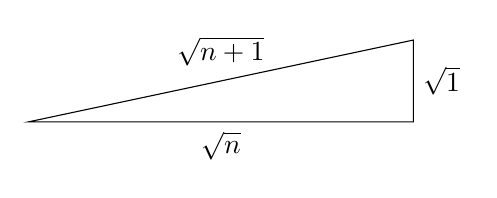
\begin{tikzpicture}
\draw (0,0) coordinate (A) -- node [above=2pt] {$\sqrt{n+1}$} (12:5) coordinate (B) -- node [right] {$\sqrt{1}$ } (B |- A) -- node [below] {$\sqrt{n}$} cycle;
\end{tikzpicture}
\selectlanguage{hebrew}
\caption{%
בניית קו באורך
$\sqrt{n+1}$}\label{fig.pyth}
\end{center}
\end{figure}

\item 
טענת בסיס: עלה הוא צומת בודד עם גובה אפס: 
$1\leq 2^{0+1}-1=1$.
הצעד האינדוקטיבי הוא: נניח ש-%
$n_h\leq 2^{h+1}-1$
והראה ש-%
$n_{h+1}\leq 2^{(h+1)+1}-1$.
כפי שניתן לראות באיור~%
\ref{fig.incomplete},
תת-עץ השמאלי ותת-עץ הימני של שורש העץ
\textbf{אינם}
באותו גובה. אולם, 
$h+1=\max(h_l,h_r)+1$,
כי הגובה של השורש הוא אחד יותר מהגובה של התת-עץ עם הגובה המקסימלי. לפי הנחת האינדוקציה:
\[
\begin{array}{l}
n_l\leq 2^{h_l+1}-1\leq 2^{\max(h_l,h_r)+1}-1 = 2^{h+1}-1\\
n_r\leq 2^{h_r+1}-1\leq 2^{\max(h_l,h_r)+1}-1 = 2^{h+1}-1\,.
\end{array}
\]
ולכן:
\[
n_{h+1} = n_l + n_r + 1 \ihle{} (2^{h+1}-1) + (2^{h+1}-1) + 1 = 2^{(h+1)+1} - 1\,.
\]

\item 
טענת בסיס: קשת אחת נושקת לשני צמתים וקיים שטח אחד שהוא כל המישור:
$1+2=1+2$.
יש שני צעדי אינדוקטיביים: אם צומת נושק לקשת אחת, מחק את הצומת והקשת. השוויון 
$s+(n+1)=(e+1)+2$
נובע מהנחת האינדוקציה. אם אין צמתים כאלה אז כל קשת הוא חלק ממסלול מעגלי. מחיקת הקשת משאירה את מספר הצמתים ללא שינוי, מורידה ב-%
$1$
את מספר הקשתות ומורידה את מספר השטחים גם הוא ב-%
$1$.
השוויון
$(s-1)+n=(e-1)+2$
נובע מהנחת האינדוקציה.

%%%%%%%%%%%%%%%%%%%%%%%%%%%%%%%%%%%%%%%%%%%%%%%%%%%%%%%%%%%%%%%%%%%

\item 
אם 
$n$
מתחלק ב-%
$3$
סיימנו. אחרת,
$n=3k+1$
או
$n=3k+2$.
מכאן:
\[
n+1=3k+2+1=3k+3
\]
או:
\[
n+2=3k+1+2=3k+3
\]
מתחלק ב-%
$3$.

\item
הוכחה ללא אינדוקציה:
\begin{eqnarray*}
(x-1)\sum_{i=0}^{i=n}x^i &=& x\sum_{i=0}^{i=n}x^i - \sum_{i=0}^{i=n}x^i\\
&=&x^{n+1} + \sum_{i=1}^{i=n}(x^i-x^i) -x^0\\
&=&x^{n+1} - 1\,.
\end{eqnarray*}

הוכחה באינדוקציה: טענת בסיס:
$x^0-1=0$
מתחלק על ידי כל פולינום. הצעד האינדוקטיבי:
\[
x^{n+1} - 1 = x^{n+1} -x^n + x^n - 1= x^n(x-1) + (x^n-1)\,.
\]
ברור שהגורם הראשון מתחלק ב-%
$x-1$
ולפי הנחת האינדוקציה גם הגורם השני מתחלק ב-%
$x-1$.

\item
בצעד האינדוקטיבי עבור
$n+1$,
השתמשנו ב-%
$a^{n}=1$
שהיא נוסחה נכונה, אבל השתמשנו גם ב-%
$a^{n-1}=1$
u-%
$a^{n-2}=1$,
שאינן נכונות אלא אם נוכיח טענות בסיס נוספות
$a^{-1}=1$
ו-%
$a^{-2}=1$,
לכל
$a\geq 1$.
אולם, שתי הטענות אינן נכונות.

\item
השתמשנו בהנחת האינדוקציה עבור קבוצות שונות עם
$n$
איברים:
$s_1,s_2,\ldots,s_{n-1},s_n$
ו-%
$s_1,s_2,\ldots,s_{n-1},s_{n+1}$.
אולם, קבוצות אלו שונות רק אם
$n\geq 3$
ולא הוכחנו טענת בסיס עבור 
$n=2$.
כמובן שזה בלתי אפשרי כי ייתכן שתלמיד
$s_1$
צבע את שיערו ירוק ותלמידה
$s_2$
צבעה את שיערה כחול.

%%%%%%%%%%%%%%%%%%%%%%%%%%%%%%%%%%%%%%%%%%%%%%%%%%%%%%%%%%%%%%%%%%%

\item
הנוסחה
$A=p$
ספיקה אם ורק אם הנוסחה
\[
A'= (p \vee q \vee r) \;\wedge\; (p \vee \neg q \vee r) \;\wedge\; (p \vee q \vee \neg r) \;\wedge\; (p \vee \neg q \vee \neg r).
\]
ספיקה עם אטומים חדשים 
$q$
ו-%
$r$.
ברור שאם
$A$
ספיקה אז גם 
$A'$
על ידי הצבת
$T$
ב-%
$p$.
מה קורה אם 
$A'$
ספיקה? אם ההצבה כוללת הצבה של 
$T$
ל-%
$p$
גם
$A$
ספיקה. אחרת
$p$
קיבל הצבה של
$F$.
מה עם ההצבות ל-%
$q$
ו-%
$r$?
אחד מ:
\[
q \vee r, \neg q \vee r,\vee q \vee \neg r, \neg q \vee \neg r
\]
יקבל ערך
$F$.
לכן
$A'$
ספיקה רק אם 
$p$
מקבל הצבה
$T$.
הוכחה דומה קיימת עבור הליטרל
$\neg p$.

\item
יהי
$A\stackrel{*}{\Rightarrow} w$.
קיימים שלושה מקרים בהתאם לכלל היצירה הראשון בגזירה. אם הכלל היה
$A \rightarrow a$,
ברור ש-%
$\#a=\#b+1$
כי
$1=0+1$.
אם הכלל היה
$A\rightarrow aS$,
לפי הנחת האינדוקציה בנוסחה~%
\ref{eq.formal1}, $S\stackrel{*}{\Rightarrow} w'$
כך ש-%
$\#a=\#b$
ב-%
$w'$.
לכן
$\#a=\#b+1$
ב-%
$w$.
אם
$A\rightarrow bAA$,
אז נשתמש פעמיים בהנחת האינדוקציה
\ref{eq.formal2}
ונקבל
$AA\stackrel{*}{\Rightarrow} w'$
כך ש-%
$\#a=\#b+2$
ב-%
$w'$,
ולכן
$\#a=\#b+1$
ב-%
$w$.
ההוכחה עבור נוסחה~%
\ref{eq.formal3}
היא סימטרית.

ההוכחה בכיוון הנגדי: יהי
$S\stackrel{*}{\Rightarrow} w$
כך ש-%
$\#a=\#b$
ב-%
$w$.
נניח שהכלל הראשון בגזירה היה
$S\rightarrow aB$.
מכאן של המחרוזת
$w'$
שנגזרת מ-%
$B$
יש
$\#a+1=\#b$. 
לפי הנחת האינדוקציה בנוסחה~%
\ref{eq.formal3},
קיימת גזירה
$B\stackrel{*}{\Rightarrow} w'$,
כך שיש גזירה
$S \rightarrow aB \stackrel{*}{\Rightarrow} w$.
המקרה שהגזירה הראשונה היא
$S\rightarrow bA$
דומה, כמו ההוכחות של הכיוונים הנגדיים של הנוסחות~%
\ref{eq.formal2}
ו~%
\ref{eq.formal3}.

%%%%%%%%%%%%%%%%%%%%%%%%%%%%%%%%%%%%%%%%%%%%%%%%%%%%%%%%%%%%%%%%%%%

\item
למה 2: לכל 
$i$,
האיברים ב-%
$B_i$
ממויינים
\textbf{וגם}
כל האיברים ב-%
$A_i$
גדולים או שווים לכל האיברים ב-%
$B_i$.

טענת בסיס: 
$B_0$
היא קבוצה ריקה והטענה ריקה. הצעד האינדוקטיבי: הנחת האינדוקציה היא שלמה~2 נכונה עבור 
$A_i$
ו-%
$B_i$.
לכן, כאשר מוסיפים את האיבר
$a_i$
לסוף של
$B_i$
כדי לקבל
$B_{i+1}$,
הוא גדול או שווה לכל האיברים ב-%
$B_i$, 
ומכאן ש-%
$B_{i+1}$
ממויינת. כל האיברים של
$A_{i+1}$
גדולים או שווים לכל האיברים של
$B_{i+1}$: \L{(1)}
לפי הנחת האינדוקציה האם כבר היו גדולים אל שווה לכל האיברים ב-%
$B_i$,
ו-%
\L{(2)}
$a_i$
היה האיבר הקטן ב-%
$A_i$
כך שהם גדולים או שווים ל-%
$a_i$
שהתווסף ל-%
$B_i$
כדי לקבל
$B_{i+1}$.

\item
טענת בסיס: הערך התחילי של המשתנה 
\L{\texttt{sem}}
הוא
$1$
ו-
$\#\mathit{CS}=0$
כי אין אף תהליך בקטע הקריטי. לפי הנחת האינדוקציה, נניח שהנוסחה נכונה. היא יכולה להפוך ללא נכונה רק אם ערכים של
$\#\mathit{CS}$
או
$\mathit{sem}$
משתנים. התהליכים סימטריים, ולכן ללא הגבלת הכלליות אפשר לבדוק רק פקודות מתהליך
\L{\texttt{p}}.
שגיאה יכולה לקרות רק אם ביצוע הפקודה
\L{\texttt{p1}}
או הפקודה
\L{\texttt{p3}}.
ביצוע
\L{\texttt{p1}}
מוסיף
$1$
לערך של
$\#\mathit{CS}$
אבל גם מחסיר 
$1$ 
מערכו של
$\mathit{sem}$.
באופן דומה, ביצוע של
\L{\texttt{p3}} 
מחסירה
$1$
מערכו של
$\#\mathit{CS}$
אבל מוסיף
$1$
לערכו של
$\mathit{sem}$.

%%%%%%%%%%%%%%%%%%%%%%%%%%%%%%%%%%%%%%%%%%%%%%%%%%%%%%%%%%%%%%%%%%%

\item 
אם
$n$
אי-זוגי,
$n-7$
זוגי, ולכן אם ניתן לבנות מספרים זוגיים גדולים ככל שנרצה, נוכל לבנות מספרים אי-זוגיים גדולים ככל שנרצה על ידי הוספת מטבע אחד של
$7$
ש"ח. ברור, שניתן לבנות מספרים שהם כפולות של
$4$, $n=4k$,
מ-%
$k$
מטבעות של
$4$
ש"ח. לכן, כל מה שנשאר הוא להוכיח שניתן לבנות מספר זוגי שאינו כפולה של
$4$.

קל להראות שהמספרים
$1,2,3,5,6,9,10,11,13,15,17$
לא ניתנים לבנייה. למשל, 
$17$
אי-זוגי, לכן חייבים להשתמש במטבע של 
$7$,
ולהשתמש בו פעם אחד בלבד כי לא ניתן לייצר
$17-2\cdot 7=3$.
אבל
$17-7=10$
לא מתחלק ב-%
$4$
ולכן הבנייה בלתי אפשרית.

נוכיח באינדוקציה שניתן לבנות כל מספר זוגי גדול או שווה ל-%
$18$
שלא מתחלק ב-%
$4$.

טענת בסיס:
$18=2\cdot 7 + 4$.

מספרים זוגיים שלא ניתן לחלק ב-%
$4$
ניתן לבטא כ-%
$2(2k+1)$.
הצעד האינדוקטיבי:
\[
2(2(n+1)+1) = 4n+6 = (4n+2)+4.
\]
לפי הנחת האינדוקציה, ניתן לבנות
$4n+2=2(2n+1)$.
נוסיף מטבע אחד של
$4$
ונקבל
$2(2(n+1)+1)$.

\item
טענת הבסיס: השבר
$\frac{a}{b}$
הוא שבר יסודי
$a=1$.
הצעד האינדוקטיבי הוא שהטענה נכונה עבור כל שבר שהוא קטן מ-%
$\frac{a}{b}$.
לפי הנחת האינדוקציה והבחירה של
$\frac{1}{q} < \frac{a}{b}$,
ניתן לבטא את
\[
\left( \frac{a}{b} - \frac{1}{q} \right) < \frac{a}{b}
\]
כסכום של שברים יסודיים. מכאן שניתן לבטא את:
\[
\frac{a}{b} = \frac{1}{q} + \left( \frac{a}{b} - \frac{1}{q} \right)
\]
כסכום של שברים יסודיים.

אם
$\frac{1}{q}$
הוא השבר היסודי
\textbf{הגדול ביותר}
שהוא פחות מ-%
$\frac{a}{b}$,
אזי
$\frac{a}{b} < \frac{1}{q-1}$,
ולכן
$aq-b < a$
ו-%
\[\left( \frac{a}{b} - \frac{1}{q} \right) = \frac{aq-b}{bq} = (aq-b)\cdot \frac{1}{b}\cdot\frac{1}{q} < a\cdot\frac{1}{b}\cdot\frac{1}{q}<\frac{1}{q}\,,
\]
כי
$\frac{a}{b}$
הוא שבר אמיתי. מכאן שאף אחד מהשברים היסודים בסכום המבטא את
$\left( \frac{a}{b} - \frac{1}{q} \right)$
יכול להיות גדול או שווה ל-%
$\frac{1}{q}$.

\item
נוכיח קודם ש-%
$\phi^2=\phi+1$:
\vspace*{-8pt}
\begin{eqnarray*}
\phi^2 &=& \left(\frac{1+\sqrt{5}}{2}\right)^2\\
&=& \frac{1}{4} + \frac{2\sqrt{5}}{4} + \frac{5}{4}\\
&=& \frac{2}{4} + \frac{2\sqrt{5}}{4} + \frac{4}{4}\\
&=& \frac{1+2\sqrt{5}}{2} + 1\\
&=&\phi + 1\,.
\end{eqnarray*}
ההוכחה של
$\bar{\phi}^2=\bar{\phi}+1$
דומה.

טענת הבסיס עבור
$n=1$
היא:
\[
\frac{\phi^1 - \bar{\phi}^1}{\sqrt{5}}=\frac{(1+\sqrt{5})/2-(1-\sqrt{5})/2}{\sqrt{5}}=\frac{2\sqrt{5}}{2\sqrt{5}}=1\,.
\]
נניח את הנחת האינדוקציה לכל
$k\leq n$.
הצעד האינדוקטיבי הוא:
\begin{eqnarray*}
\phi^n - \bar{\phi}^n &=& \phi^2\phi^{n-2} - \bar{\phi}^2\bar{\phi}^{n-2}\\
&=&(\phi+1)\phi^{n-2} - (\bar{\phi}+1)\bar{\phi}^{n-2}\\
&=&(\phi^{n-1} - \bar{\phi}^{n-1}) + (\phi^{n-2} - \bar{\phi}^{n-2})\\
&\ih&\sqrt{5}f_{n-1} + \sqrt{5}f_{n-2}\,,
\end{eqnarray*}
לכן
\[
\frac{\phi^n - \bar{\phi}^n}{\sqrt{5}} = f_{n-1} + f_{n-2} = f_n\,.
\]

\item
הוכחת החוק של
\L{Pascal}:
\begin{eqnarray*}
{n \choose k} + {n \choose k+1} &=& \frac{n!}{k!(n-k)!} + \frac{n!}{(k+1)!(n-(k+1))!}\\
&=&\frac{n![(k+1)+(n-k)]}{(k+1)!(n-k)!}\\
&=&\frac{n!(n+1)}{(k+1)!(n-k)!}\\
&=&\frac{(n+1)!}{(k+1)!((n+1)-(k+1))!}\\
&=&{n+1 \choose k+1}\,.
\end{eqnarray*}
טענת בסיס:
\[
f_1 = 1 = {1 \choose 0} = \frac{1!}{0!(1-0)!}\,.
\]
הצעד האינדוקטיבי הוא:
\begin{eqnarray*}
f_{n-1} + f_{n-2} &\ih& {n-1 \choose 0} + {n-2 \choose 1} + {n-3 \choose 2} + {n-4 \choose 3} + \cdots\\
&&\hspace{5em}{n-2 \choose 0} + {n-3 \choose 1} + {n-4 \choose 2} + \cdots\\
&=&{n-1 \choose 0} + {n-1 \choose 1} + {n-2 \choose 2} + {n-3 \choose 3} + \cdots\\
&=&{n \choose 0} + {n-1 \choose 1} + {n-2 \choose 2} + {n-3 \choose 3} + \cdots.
\end{eqnarray*}
השוויון האחרון משתמש ב-:
\[
{k \choose 0} = \frac{k!}{0!(k-0)!} = 1
\]
עבור כל
$k$.

\end{enumerate}
